\documentclass{article}
\usepackage[utf8]{inputenc}
\usepackage{xcolor}
\usepackage{graphicx}
\title{BME 646/ ECE695DL: Homework 3}
\author{Chengjun Guo} 
\date{7 Feb 2022}


\begin{document}
\maketitle
\section{Introduction}
This homework is to implement an optimization of SGD based approach to update the values of the parameters.
\section{Methodology}
In this homework, I created a new class to overwrite the parent class's run training loop function and the backward parameter updating function. Setting up two other class variables to keep track of the previous iteration.

\section{Implementation and Results}
\subsection{two saved figs}
one neuron:\\
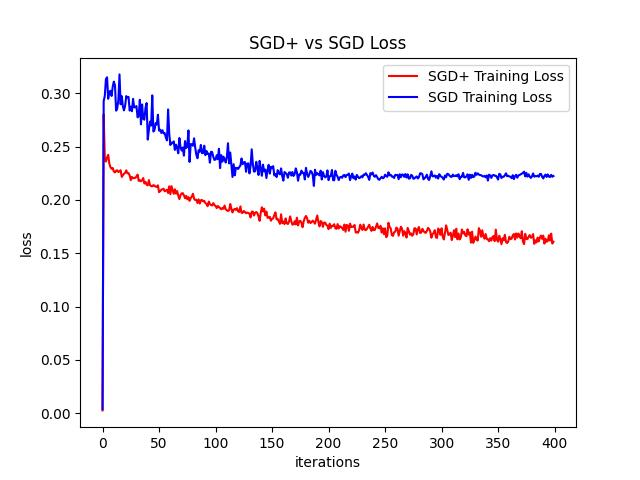
\includegraphics[scale=0.8]{one_neuron_loss.jpg}\\
multi neuron:\\
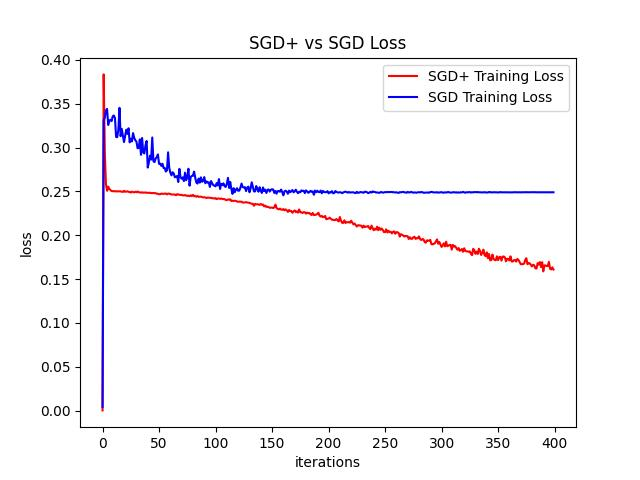
\includegraphics[scale=0.8]{multi_neuron_loss.jpg}
\subsection{one neuron modified code}
\textcolor{red}{\rule[-0.3in]{6.1in}{0.03in}}\\
\vspace{-0.05in}
\begin{verbatim}
#!/usr/bin/env python

##  one_neuron_classifier.py

"""
A one-neuron model is characterized by a single expression that you see in the value
supplied for the constructor parameter "expressions".  In the expression supplied, the
names that being with 'x' are the input variables and the names that begin with the
other letters of the alphabet are the learnable parameters.
"""

import sys,os,os.path
import numpy as np
import re
import operator
import math
import random
import torch
from collections import deque
import copy
import matplotlib.pyplot as plt
import networkx as nx


seed = 0
random.seed(seed)
np.random.seed(seed)

from ComputationalGraphPrimer import *


class ComputationalGraphPrimerPlus(ComputationalGraphPrimer):
    def run_training_loop_one_neuron_model(self, training_data, momentum_coe):
        """
        The training loop must first initialize the learnable parameters.  Remember, these are the
        symbolic names in your input expressions for the neural layer that do not begin with the
        letter 'x'.  In this case, we are initializing with random numbers from a uniform distribution
        over the interval (0,1).
        """
        self.vals_for_learnable_params = {param: random.uniform(0,1) for param in self.learnable_params}
        self.bias = random.uniform(0,1)
        self.gamma = momentum_coe
        self.prev_grad = {param: 0 for param in self.learnable_params}
        self.prev_bias = 0
        
        class DataLoader:
            """
            The data loader's job is to construct a batch of randomly chosen samples from the
            training data.  But, obviously, it must first associate the class labels 0 and 1 with
            the training data supplied to the constructor of the DataLoader.   NOTE:  The training
            data is generated in the Examples script by calling 'cgp.gen_training_data()' in the
            ****Utility Functions*** section of this file.  That function returns two normally
            distributed set of number with different means and variances.  One is for key value '0'
            and the other for the key value '1'.  The constructor of the DataLoader associated a'
            class label with each sample separately.
            """
            def __init__(self, training_data, batch_size):
                self.training_data = training_data
                self.batch_size = batch_size
                self.class_0_samples = [(item, 0) for item in self.training_data[0]]
                self.class_1_samples = [(item, 1) for item in self.training_data[1]]
            def __len__(self):
                return len(self.training_data[0]) + len(self.training_data[1])
            def _getitem(self):
                cointoss = random.choice([0,1])
                if cointoss == 0:
                    return random.choice(self.class_0_samples)
                else:
                    return random.choice(self.class_1_samples)
            def getbatch(self):
                batch_data,batch_labels = [],[]
                maxval = 0.0
                for _ in range(self.batch_size):
                    item = self._getitem()
                    if np.max(item[0]) > maxval:
                        maxval = np.max(item[0])
                    batch_data.append(item[0])
                    batch_labels.append(item[1])
                batch_data = [item/maxval for item in batch_data]
                batch = [batch_data, batch_labels]
                return batch

        data_loader = DataLoader(training_data, batch_size=self.batch_size)
        loss_running_record = []
        i = 0
        avg_loss_over_literations = 0.0
        for i in range(self.training_iterations):
            data = data_loader.getbatch()
            data_tuples = data[0]
            class_labels = data[1]
            y_preds, deriv_sigmoids =  self.forward_prop_one_neuron_model(data_tuples)
            loss = sum([(abs(class_labels[i] - y_preds[i]))**2 for i in range(len(class_labels))])
            loss_avg = loss / float(len(class_labels))
            avg_loss_over_literations += loss_avg
            if i%(self.display_loss_how_often) == 0:
                avg_loss_over_literations /= self.display_loss_how_often
                loss_running_record.append(avg_loss_over_literations)
                print("[iter=%d]  loss = %.4f" %  (i+1, avg_loss_over_literations))
                avg_loss_over_literations = 0.0
            y_errors = list(map(operator.sub, class_labels, y_preds))
            y_error_avg = sum(y_errors) / float(len(class_labels))
            deriv_sigmoid_avg = sum(deriv_sigmoids) / float(len(class_labels))
            data_tuple_avg = [sum(x) for x in zip(*data_tuples)]
            data_tuple_avg = list(map(operator.truediv, data_tuple_avg,
                                     [float(len(class_labels))] * len(class_labels) ))
            self.backprop_and_update_params_one_neuron_model(y_error_avg, data_tuple_avg, deriv_sigmoid_avg)
        return loss_running_record
        
    def backprop_and_update_params_one_neuron_model(self, y_error, vals_for_input_vars, deriv_sigmoid):
        """
        As should be evident from the syntax used in the following call to backprop function,

           self.backprop_and_update_params_one_neuron_model( y_error_avg, data_tuple_avg, deriv_sigmoid_avg)
                                                                     ^^^             ^^^                ^^^
        the values fed to the backprop function for its three arguments are averaged over the training
        samples in the batch.  This in keeping with the spirit of SGD that calls for averaging the
        information retained in the forward propagation over the samples in a batch.

        See Slides 103 through 108 of Week 3 slides for the logic implemented  here.
        ^^^^^^^^^^^^^^^^^^^^^^^^^^^^^^^^^^^^^^^^^^^^^^^^^^^^^^^^^^^^^^^^^^^^^^^^^^^^
        """
        input_vars = self.independent_vars
        vals_for_input_vars_dict =  dict(zip(input_vars, list(vals_for_input_vars)))
        vals_for_learnable_params = self.vals_for_learnable_params
        for i,param in enumerate(self.vals_for_learnable_params):
            ## calculate the next step in the parameter hyperplane
            grad = y_error * vals_for_input_vars_dict[input_vars[i]] * deriv_sigmoid
            step = self.learning_rate * grad + self.gamma * self.prev_grad[param]
            self.prev_grad[param] = step
            self.vals_for_learnable_params[param] += step
        grad = y_error * deriv_sigmoid
        self.prev_bias = self.gamma * self.prev_bias + self.learning_rate * grad
        self.bias += self.prev_bias    ## the step to take for the bias

cgp = ComputationalGraphPrimerPlus(
               one_neuron_model = True,
               expressions = ['xw=ab*xa+bc*xb+cd*xc+ac*xd'],
               output_vars = ['xw'],
               dataset_size = 5000,
               learning_rate = 1e-3,
#               learning_rate = 5 * 1e-2,
               training_iterations = 40000,
               batch_size = 8,
               display_loss_how_often = 100,
               debug = True,
      )

cgp.parse_expressions()
#cgp.display_network1()
cgp.display_network2()
training_data = cgp.gen_training_data()
loss = cgp.run_training_loop_one_neuron_model(training_data, 0.0)
loss_plus = cgp.run_training_loop_one_neuron_model(training_data, 0.99)

plt.figure()
plt.ylabel('loss')
plt.xlabel('iterations')
plt.title('SGD+ vs SGD Loss')
plt.plot(loss_plus, label = 'SGD+ Training Loss', color='r')
plt.plot(loss, label = 'SGD Training Loss', color='b')
plt.legend()
#plt.show()
plt.savefig("one_neuron_loss.jpg")

\end{verbatim}
\vspace{-0.45in}
\textcolor{red}{\rule[-0.3in]{6.1in}{0.03in}}\\
\subsection{multi neuron modified code}
\textcolor{red}{\rule[-0.3in]{6.1in}{0.03in}}\\
\vspace{-0.05in}
\begin{verbatim}
#!/usr/bin/env python

##  one_neuron_classifier.py

"""
A one-neuron model is characterized by a single expression that you see in the value
supplied for the constructor parameter "expressions".  In the expression supplied, the
names that being with 'x' are the input variables and the names that begin with the
other letters of the alphabet are the learnable parameters.
"""

import sys,os,os.path
import numpy as np
import re
import operator
import math
import random
import torch
from collections import deque
import copy
import matplotlib.pyplot as plt
import networkx as nx


seed = 0
random.seed(seed)
np.random.seed(seed)

from ComputationalGraphPrimer import *


class ComputationalGraphPrimerPlus(ComputationalGraphPrimer):
    def run_training_loop_one_neuron_model(self, training_data, momentum_coe):
        """
        The training loop must first initialize the learnable parameters.  Remember, these are the
        symbolic names in your input expressions for the neural layer that do not begin with the
        letter 'x'.  In this case, we are initializing with random numbers from a uniform distribution
        over the interval (0,1).
        """
        self.vals_for_learnable_params = {param: random.uniform(0,1) for param in self.learnable_params}
        self.bias = random.uniform(0,1)
        self.gamma = momentum_coe
        self.prev_grad = {param: 0 for param in self.learnable_params}
        self.prev_bias = 0
        
        class DataLoader:
            """
            The data loader's job is to construct a batch of randomly chosen samples from the
            training data.  But, obviously, it must first associate the class labels 0 and 1 with
            the training data supplied to the constructor of the DataLoader.   NOTE:  The training
            data is generated in the Examples script by calling 'cgp.gen_training_data()' in the
            ****Utility Functions*** section of this file.  That function returns two normally
            distributed set of number with different means and variances.  One is for key value '0'
            and the other for the key value '1'.  The constructor of the DataLoader associated a'
            class label with each sample separately.
            """
            def __init__(self, training_data, batch_size):
                self.training_data = training_data
                self.batch_size = batch_size
                self.class_0_samples = [(item, 0) for item in self.training_data[0]]
                self.class_1_samples = [(item, 1) for item in self.training_data[1]]
            def __len__(self):
                return len(self.training_data[0]) + len(self.training_data[1])
            def _getitem(self):
                cointoss = random.choice([0,1])
                if cointoss == 0:
                    return random.choice(self.class_0_samples)
                else:
                    return random.choice(self.class_1_samples)
            def getbatch(self):
                batch_data,batch_labels = [],[]
                maxval = 0.0
                for _ in range(self.batch_size):
                    item = self._getitem()
                    if np.max(item[0]) > maxval:
                        maxval = np.max(item[0])
                    batch_data.append(item[0])
                    batch_labels.append(item[1])
                batch_data = [item/maxval for item in batch_data]
                batch = [batch_data, batch_labels]
                return batch

        data_loader = DataLoader(training_data, batch_size=self.batch_size)
        loss_running_record = []
        i = 0
        avg_loss_over_literations = 0.0
        for i in range(self.training_iterations):
            data = data_loader.getbatch()
            data_tuples = data[0]
            class_labels = data[1]
            y_preds, deriv_sigmoids =  self.forward_prop_one_neuron_model(data_tuples)
            loss = sum([(abs(class_labels[i] - y_preds[i]))**2 for i in range(len(class_labels))])
            loss_avg = loss / float(len(class_labels))
            avg_loss_over_literations += loss_avg
            if i%(self.display_loss_how_often) == 0:
                avg_loss_over_literations /= self.display_loss_how_often
                loss_running_record.append(avg_loss_over_literations)
                print("[iter=%d]  loss = %.4f" %  (i+1, avg_loss_over_literations))
                avg_loss_over_literations = 0.0
            y_errors = list(map(operator.sub, class_labels, y_preds))
            y_error_avg = sum(y_errors) / float(len(class_labels))
            deriv_sigmoid_avg = sum(deriv_sigmoids) / float(len(class_labels))
            data_tuple_avg = [sum(x) for x in zip(*data_tuples)]
            data_tuple_avg = list(map(operator.truediv, data_tuple_avg,
                                     [float(len(class_labels))] * len(class_labels) ))
            self.backprop_and_update_params_one_neuron_model(y_error_avg, data_tuple_avg, deriv_sigmoid_avg)
        return loss_running_record
        
    def backprop_and_update_params_one_neuron_model(self, y_error, vals_for_input_vars, deriv_sigmoid):
        """
        As should be evident from the syntax used in the following call to backprop function,

           self.backprop_and_update_params_one_neuron_model( y_error_avg, data_tuple_avg, deriv_sigmoid_avg)
                                                                     ^^^             ^^^                ^^^
        the values fed to the backprop function for its three arguments are averaged over the training
        samples in the batch.  This in keeping with the spirit of SGD that calls for averaging the
        information retained in the forward propagation over the samples in a batch.

        See Slides 103 through 108 of Week 3 slides for the logic implemented  here.
        ^^^^^^^^^^^^^^^^^^^^^^^^^^^^^^^^^^^^^^^^^^^^^^^^^^^^^^^^^^^^^^^^^^^^^^^^^^^^
        """
        input_vars = self.independent_vars
        vals_for_input_vars_dict =  dict(zip(input_vars, list(vals_for_input_vars)))
        vals_for_learnable_params = self.vals_for_learnable_params
        for i,param in enumerate(self.vals_for_learnable_params):
            ## calculate the next step in the parameter hyperplane
            grad = y_error * vals_for_input_vars_dict[input_vars[i]] * deriv_sigmoid
            step = self.learning_rate * grad + self.gamma * self.prev_grad[param]
            self.prev_grad[param] = step
            self.vals_for_learnable_params[param] += step
        grad = y_error * deriv_sigmoid
        self.prev_bias = self.gamma * self.prev_bias + self.learning_rate * grad
        self.bias += self.prev_bias    ## the step to take for the bias

cgp = ComputationalGraphPrimerPlus(
               one_neuron_model = True,
               expressions = ['xw=ab*xa+bc*xb+cd*xc+ac*xd'],
               output_vars = ['xw'],
               dataset_size = 5000,
               learning_rate = 1e-3,
#               learning_rate = 5 * 1e-2,
               training_iterations = 40000,
               batch_size = 8,
               display_loss_how_often = 100,
               debug = True,
      )

cgp.parse_expressions()
#cgp.display_network1()
cgp.display_network2()
training_data = cgp.gen_training_data()
loss = cgp.run_training_loop_one_neuron_model(training_data, 0.0)
loss_plus = cgp.run_training_loop_one_neuron_model(training_data, 0.99)

plt.figure()
plt.ylabel('loss')
plt.xlabel('iterations')
plt.title('SGD+ vs SGD Loss')
plt.plot(loss_plus, label = 'SGD+ Training Loss', color='r')
plt.plot(loss, label = 'SGD Training Loss', color='b')
plt.legend()
#plt.show()
plt.savefig("one_neuron_loss.jpg")

\end{verbatim}
\vspace{-0.45in}
\textcolor{red}{\rule[-0.3in]{6.1in}{0.03in}}\\

\section{Lessons Learned}
Sometimes big problem can be solved by effective simple algorithm. Adding a momentum for each single iteration can help converging with many iterations.
\section{Suggested Enhancements}
For this homework, making modification to the ComputationalGraphPrimer could make the code more succinct.
\end{document}